\documentclass{scrartcl}
% \documentstyle{article}
\usepackage{comment}
\usepackage{amsmath}
\usepackage{caption}
\usepackage{graphicx}
\usepackage{subfig}
\begin{comment}

\end{comment}
\usepackage{xcolor}
\newcommand\todo[1]{\textit{\textcolor{red}{#1}}}

\DeclareCaptionType{mycapequ}[][List of equations]
\captionsetup[mycapequ]{labelformat=empty}

\providecommand{\comm}[1]{{\bf[ #1 ]}}
\providecommand{\commd}[1]{\comm{D: {#1}}}

\begin{document} 
\title{Item Reponse Theory in Intelligent Tutoring Systems}
\subtitle{Can IRT-based Learner Models used in an IRT Goals?}

\author{Lieuwe Rekker}
\maketitle
\nocite{labelcombi}
\nocite{lftransfer}
\nocite{importance}
\nocite{knowledgeproblem}
\nocite{modelreview}
\nocite{eirt}
\nocite{pfa}
\nocite{ktpfa}
\nocite{skillcombi}
\nocite{lfa}
\nocite{blackart}
\nocite{hambleton}
\nocite{bridge}
\nocite{ct}
\nocite{algebra}
\nocite{assessment}

%\listofmycapequs

\section{Introduction}
Intelligent Tutor Systems (ITS) are computer programs in which students do exercises. The exercises themselves are similar to the pen and paper exercises that students would do from textbooks. ITSs provide some advantages and new opportunities though. For one the ITS can provide direct and tailored feedback to the student and adapt the order in which exercises are presented to the student. One of the opportunities of these ITS systems is that they can easily record the student data on whether or not students answered questions correctly. This has lead to more and more datasets of student interaction with ITSs being available for research.

This data has given rise to learner (or skill) models that as an input use the data of what student, asked what question and as an output provide a probability of whether the student answered the question correctly or not. The focus of these models is mostly on how well they make their predictions as this is a metric that is directly observable in the data. Unfortunately this draws attention away from other uses that such a model could be put towards such as assessment.

Assessment has been a hot item in education for a long time and has received renewed attention since the implementation of the 
'no child left behind' act in the US in 2001. A problem with a focus on assessment is that it takes time away from education. It would therefor be nice if the ITSs that are used to teach children could also assess them while doing so.

In psychology and more specifically psychometrics, assessment has been an important subject of study, which has led to the development of Item Response Theory (IRT). IRT shows some resemblance to the learner models mentioned above: the data is from tests where students also answer questions and answers are recorded. The IRT models look like the above learner models in that they too produce predictions for student answers. The interest of the model is not in these predictions though, but on whether the values the model assigns to student skill are correct. Since this student skill is hard to determine IRT has developed a toolbox with which to determine if the model works correctly on particular data and can even be used to help identify bad test items. 

Data from ITSs differs from the data from tests, but nevertheless learner models have been developed based on the models used in IRT. These models have mostly been evaluated from the 'correct prediction' perspective and not the IRT toolkit which is more concerned with estimating student level and test quality.

In this thesis IRT based learner models will be evaluated from an IRT perspective to gain an idea of whether these IRT based model can be used in similar ways to IRT models such as establishing the level of student skill and identifying poor questions. 

\section{Models}
\subsection{IRT Models}
For every question asked an IRT model uses the student $s$ and the item $i$ as input and returns a probability $P$ that the question is answered correctly. The function at the basis of providing this probability is the logistic ogive function (see formula \ref{eq:logistic}). Each student has exactly one parameter associated with them which represents the ability of the student and is here named skill and indicated by $\theta$. This parameter is generally the parameter of highest interest in tests as it can be used to order the level of skill of the different students. The number of parameters associated with items and how all these are combined into $x$ differs per particular model and is discussed in the following paragraphs.
\begin{equation}
\label{eq:logistic}
\sigma(x) = \frac{1}{1+e^{-x}}
\end{equation}

\subsubsection{1PL or Rasch Model}
\label{sec:1PL}
The 1PL model, also known as the Rasch model has one parameter ($b$) per item, which stands for the difficulty of the item. The entire formula for a question's probability of a correct answer is $P(s,i) = \sigma(\theta_{s} - b_{i})$. This means that when the skill of the student and the difficulty of the item are on a par, the student has a probability of .5 to answer the question correctly. Note that there exists an indeterminacy issue with this model: one can have the same results while changing the parameter values by increasing or decreasing all $\theta$ and $b$ by the same amount. This problem is generally solved by setting the average $\theta$ to 0.

\subsubsection{2PL Model}
The 2PL model expands the 1PL model with the parameter $a$ which is called the discrimination of the item. The 2PL then looks like this: $P(s,i) = \sigma(a_{i} (\theta_{s} - b_{i}))$ The term discrimination comes from the fact that a high discrimination causes $P$ to change quickly when $|(\theta_{s} - b_{i})|$ is small and thus the performance of students who are close in skill can be more easily distinguished. The flip-side here is that when $|(\theta_{s} - b_{i})|$ isn't small, $P$ will more quickly drop to 0 or rise to 1, concealing any difference between skill levels at those levels. Note that for this model not only can $\theta$ and $b$ be increased or decreased by the same amount, but all $a$ can be scaled up or down as long as all $\theta$ and $b$ are scaled down or up respectively by the same factor. This problem is generally solved by setting the average $\theta$ to 0 and its variance to 1. 

\subsubsection{3PL Model}
The final IRT model discussed here is the 3PL model which adds a chance parameter $c$. This model takes into account that on occasion the student could answer a question correctly by taking a (educated) guess. This phenomenon is most prevalent in multiple choice tests where the chances of correctly guessing the answer are obvious and relatively very high. The model effectively changes the lowest probability to the level of $c$ and the space between $c$ and $1$ is rescaled accordingly leading to formula \ref{eq:3PL}. This model suffers from the same identifiability issues as the 2PL model. In this thesis this model is left out of consideration, as none of the learning models are based on it and none of the data is multiple choice and will thus not be mentioned again. 

\begin{equation}
\label{eq:3PL}
P(s,i)= c_{i} + \frac{1-c_{i}}{1+e^{-a_{i}(\theta_{s} - b_{i})}}
\end{equation}

\subsubsection{Fitting the Models}
The above paragraphs have discussed what the parameters are taken to represent and how they are used in the model. None of these parameters are directly observable (i.e. they are latent) and thus are not directly obtained from observations. Instead the observed answers to the questions asked and the probability that the those answers would be generated by the model are used. The parameters are given those values at which the likelihood that the observed answers arise from the model is maximized. The likelihood of the answer to a single question is the probability that that answer is seen according to the model. Thus if the answer is correct, the likelihood for that answer is $P$, while if the question is answered incorrectly the likelihood is $1-P$. By taking the product of the likelihoods of every data point the likelihood of the entire dataset is determined, which gives formula \ref{eq:likely}.

\begin{equation}
\label{eq:likely}
L=\prod_{d \in D} P_{d}^{t_d}  (1- P_{d})^{1-t_d}
\end{equation}

In the 1PL model $x$ is linear in the parameters, which makes maximizing the likelihood quite straightforward: logistic regression can be directly applied to this problem. In the 2PL $x$ is bi-linear and thus logistic regression can not be applied directly. Instead values for student parameters are fixed (making $x$ linear again), logistic regression is applied, the found item parameter values are then kept fixed to find the values for the student parameters. This procedure is repeated until the likelihood of the data is (nearly) the same in consecutive runs of logistic regression. For more detailed information on logistic regression and how it is used here, please refer to appendix \ref{app:math}.

Note that this model can go haywire if a student answers all his questions correctly or incorrectly (the students ability will run to plus or minus infinitely respectively) or if an item is always answered correctly  or incorrectly. To prevent this issue these are removed from the data before fitting.

\subsubsection{Information Function}
\label{sec:inherent}
All IRT models are stochastic in nature: even when the probability of a correct answer is 90\%, an incorrect answer is still expected in 10\% of the cases. This means that even if data would be noiselessly generated by the model, some variation will be present if we generate a dataset multiple times for the same set of questions. This also means that even though the parameters used to generate this data are exactly the same, the parameters found in the fitting process will be different for each generated dataset. This is some variance in the found parameters that will last even if the data is noiseless.  

To justify conclusions drawn from application of IRT, these variance are approximated by information functions. Baker \cite{basicbaker} describes an item information function as a function based on a set of items (with known parameters) that returns the variance in skill for a student that would be found if a student would answer this set of items over and over again, while every time forgetting he has seen these items. The independent variable in this item information function is the skill of the student. The reason becomes clear from a small though experiment. If a students skill is so low that he would probably give only wrong answers to the set of items, the estimates will be very inaccurate: the value of his skill could be a large negative value, but it might just as well be twice as big. Students with about average skill probably give a correct answer to about half the items, leaving far less uncertainty about their skill.

An equivalent information function can also be made for a group of students (again with known parameters) where, given parameters for an item, the variances for its parameters is given. An information function can even be defined for a set of questions where student and item parameters are obtained concurrently. Note that in all these cases only the data (the questions) are important and not the labels (the answers). The answers do influence the found variances indirectly through their influence on the fitted value of the parameters.



\subsubsection{Assessment of fit}
The issue with assessing a fitted IRT model, is that the parameter values are not directly observable. It might be possible through the use of experts to get an indication whether the parameter values are plausible, but this would at least be costly and still poses additional problems (e.g. even experts amongst each others can disagree). There is thus no easy direct way to check the values of the parameters. In \cite{hambleton} Hambleton puts forward three types recommendations of indirect evidence to inspect model fit:

\begin{quote}"[J]udgements about the fit of the model to the test data [should] be based on three types of evidence: 1. Validity of the assumptions of the model for the test data 2. Extend to which the expected properties of the model (e.g., invariance of item and ability parameters) are obtained 3. Accuracy of model predictions using real and, if appropriate, simulated test data."[p.55]
\end{quote}

The third point is most straightforward: if the predictions by the model for questions that were not used in fitting are inaccurate, the model is probably not a good fit for the data. The most important assumption the first point refers to is that of unidimensionality: the skill represented by $\theta$ should be the only skill of importance in answering the items. A good example is when some questions on a math question use difficult wording, making a high skill in math insufficient for correctly answering this item, while a student with mediocre math skill, but good language skills might answer the questions correctly. The second point and especially the mentioned example of invariance is of major importance for IRT. In Hambleton's own words: "The property of invariance of item and ability parameters is the cornerstone of IRT". Invariance means that the values obtained for items are the same (apart from the rescaling discussed) whether they are fitted on the data obtained from one group of students or another group of students and vice versa for student parameters. To test for invariance Hambleton proposes to split the students/items in two and see if the parameters of the items/students fit on the two different sets resemble each other. The method he uses for this is to plot them against each other and see if this plot produces a straight line. The property of invariance should go even further though, and he proposes to split the students/items such that the highest skilled/most difficult ones are in the same group and repeat the same procedure. He concedes that some more scatter is expected at the low and high ends of the parameter scales due to the higher inherent variance discussed in the previous section.




\subsection{IRT based learner models}
Although the models used in this research are based on the 1PL and 2PL models, there are also some important differences. The first and most obvious is that they incorporate learning, as students' skill level is expected to increase as they answer questions. To represent this, skill in the model, $\theta$, is split up in an initial part and a learned part, such that each time they answer a question the students skill increases. 
Another major difference is that the assumption that a single skill is measured, is dropped. In these models a single item can be associated with multiple skills. The name for one such skill in these models is knowledge component (KC). This means that the assumption of unidimensionality is dropped and rather that the new assumption is not that a single skill is involved, but rather that any skill that influence the answer is known within the model.

Additionally to this a subtle but major change was made to the item parameters in the model. Instead of assigning parameter values to items, value parameters are assigned to the KCs. Thus in these models an item is associated to one or more Knowledge components that have their own difficulty level etc. The items themselves no longer has parameters, only the KCs it is associated with do. From a data perspective this makes sense as the number of knowledge components is smaller than the number of items (here ranging from 8 to 1000 times as small), this greatly reduces the number of parameters that need to be fit.

\subsubsection{Learning Factor Analysis (LFA)}
\label{sec:AFM}
The LFA model (or alternatively additive factor model: AFM) has the 1PL model as its basis, but extents it by introducing a learning rate as discussed in the introduction and by allowing multiple knowledge components to be associated with a single item. The combination of KCs is made by summing the learned part of knowledge and the difficulty of the KC for every KC that is linked to the item.

\begin{equation}
\label{eq:afm}
P = \sigma(\theta_{s,0} + \sum_{c \in KC_{i}}  \gamma_{c} t_{s,c} - \beta_{c})
\end{equation}

The splitting of $\theta$ leads to the introduction of an initial skill $\theta_{0}$ defined per student, a learning rate $\gamma$ defined per KC (i.e. the KC determines how fast or slow learning occurs) and a number of times that a student has seen items associated with this particular knowledge component $t_{s,c}$. Please note that in the the original LFA model $\beta$ is added. It is subtracted here to maintain similarity to the original IRT models and ensure uniformity with the other models used. This has no other effect than that the signs for $\beta$ are reversed.

The indeterminacy that can occur in the 1PL model (discussed in section \ref{sec:1PL}) is absent here when items are associated with a different number of knowledge components (which is expected). Raising $\beta$ and $\theta_{0}$ by the same amount will affect items with a different number of associated KCs differently leading to different Ps. 



\subsubsection{Performance Factor Analysis (PFA)}
\label{sec:pfa}
The PFA model is a direct extension of the LFA model. In the PFA model separate learning rates are used for questions answered correctly and questions answered incorrectly. Additionally $\theta_{0}$ is dropped. As put forward in \cite{pfa} $\theta_{0}$ is dropped because this extension is made mostly to make this model more useful in ITSs. Leaving out any student specific parameter makes the model more easily applicable to students not used in the fitting procedure. As noted in both \cite{ktpfa} and \cite{blackart}, leaving out $\theta_{s,0}$ makes parameter estimates worse. Since prediction for students who were not part of the fitting procedure is not a concern here, a model that does include $\theta_{s,0}$ (as done in \cite{ktpfa} and \cite{blackart}) is used instead of PFA and will be referred to as PFA+.

\begin{equation}
\label{eq:pfa}
P = \sigma(\theta_{s,0} \sum_{c \in KC}  \gamma_{c} g_{s,c} + \rho_{c} f_{s,c} - \beta_{c})
\end{equation}


Here $\gamma$ is the learning rate of the KC for correct answers and g is the number of questions answered correctly. $\rho$ is the learning rate of the KC for incorrect answers and f is the number of questions answered incorrectly. Just as with the LFA model above the sign for $\beta$ is reversed compared to the original representation of the model.

\subsubsection{extended Item Response Theory (eIRT)}
\label{sec:eirt}
The extended Item Response Theory model by Roijers et al \cite{eirt} is the most straightforward extension to a standard IRT model and is different from the previous two models in that it is unidimensional. It is an extension of the 2PL model and splits $\theta$ into an initial skill and a learned part. 

\begin{equation}
\label{eq:eirt}
P = \sigma(\alpha_{c} (\theta_{s,0} + \eta_{s} t_{s,c} - \beta_{c}))
\end{equation}

Although the incorporation of a learning rate is similar to the above two models, there is a major difference: here the learning rate is taken per student rather than per KC. With $\theta$ split up, it would seem that $\alpha$ obtains a slightly different meaning. For $\theta_{0}$ it still has the same discriminatory function. When looking at $\eta$ though, $\alpha$ directly impacts it as a modifier, making learning easier ($>1$) or more difficult ($<1$) for that knowledge component.

As this is a unidimensional item the problem of indeterminacy is also at play here exactly as it was in the 2PL model. This problem could be remedied in the same way as in the 2PL model.

eIRT as defined by Roijers et al does not incorporate multiple skills (KCs) per item. In order to be trained on multi-skill data and to be similar to the other models \ref{eq:sumeirt} will be used as a multi-skill extension of the eIRF. To distinguish this version from the original eIRT, this extended version will be denoted as seIRT. A notable difference here is that $\theta_{s,0}$ is divided by the number of KCs involved. This is because $\theta_{s,0}$ should only be added once just as in LFA/PFA, but nevertheless it should be modified by the corresponding $\alpha_{c}$s as well.

\begin{equation}
\label{eq:sumeirt}
P = \sigma(\sum_{c \in KC} \alpha_{c}(\frac{\theta_{s,0}}{|KC|} + \eta_{s} t_{s,c} - \beta_{c}))
\end{equation}

Please note that in the multidimensional case the indeterminacy where $\theta{s,0}$ and $\beta$ can both be shifted by the same amount is most likely no longer there as was described for the LFA model. The dependency between $\alpha$ and the other parameters still exists though and should still be resolved by fixing the standard deviation of $\theta_{s,0}$ to 1 and changing the other parameters accordingly.

\begin{comment}


\subsubsection{Combining knowledge components}
\label{sec:comb}
Something more can be said about the way KCs are combined. In \cite{skillcombi} Cen et al. show that in practice there is no difference in performance between an additive model (as used here) or a conjunctive model (where probabilities of individual KCs are multiplied). Nevertheless the authors already mention that this is probably the case because for most KCs $\beta < \eta_{c} t_{s,c}$, meaning that adding KCs does decrease the chance of answering the question correctly as would be expected. In their paper they already propose using a data set where ($\beta > \eta_{c} t_{s,c}$) to see if this is indeed why this way of combining KCs works well in practice.

The experiment proposed above is put to the test here. Fitting a conjunctive model is hard in practice, but generating data using one is rather straightforward. Whether a real life data set contains many questions where skills are such that $\beta < \eta_{c} t_{s,c}$ cannot be said at this point. Even if this is not the case though, it can be argued that the parameter values can be skewed slightly to ensure that this occurs. The rationale behind is, is that the fitted values obtained from the real data may be skewed towards $\beta < \eta_{c} t_{s,c}$ due to a additive model being used in the fitting process. It would then be expected though that the retrieved parameters using these values would be skewed towards $\beta < \eta_{c} t_{s,c}$ again.

In comparing seIRT's (or eIRT's) parameter values to those of LFA $\beta$ should be multiplied by $\alpha$. $\theta$ is to be multiplied by a weighted average of $\alpha$ (according to the ratio of KCs of the questions that the corresponding student has answered). Finally a weighted average of $\eta$ per KC should be taken according to the ratio of questions each student has answered containing that KC. seIRT can be compared to PFA by combining the steps above with the steps needed to compare PFA to LFA.

\end{comment}

\subsubsection{Combined Model}
The three models introduced above can all be encompassed by a more complex model.

\begin{equation}
P = \sigma(\sum_{c \in KC}\frac{\alpha_c \theta_{s,0}}{|KC|}+\eta_{s} \gamma_{c} g_{s,c} + \eta_{s}\rho_{c} f_{s,c} - \beta_{c})
\end{equation}

LFA can be obtained from this model by taking $\alpha=1$, $\eta=1$ and $\gamma=\rho$. PFA can be obtained from this model by taking $\alpha=1$, $\eta=1$ and $\theta_{0}=0$ (minus the last one for PFA+). The adapted eIRF can be obtained by taking $\gamma=\rho=\alpha$ and realizing that $\beta$ already incorporates $\alpha$. It suffers from the same indeterminacy problem as the seIRT model, which can be dealt with in the same way.

\subsubsection{Model issue}
\todo{Somehow it seems to me that it is a major issue that these models are inconsistent: Students have only a single initial skill, while after learning skills diverge. This is rather odd as forgetting this past and fitting the model again would result in all these different levels being dumped into a single skill again.}


\section{Related work}
\label{sec:RW}
\subsection{LFA and PFA Model Backgrounds}
Learning factor analysis (LFA) is a method of analysis put forward in \cite{lfa} to obtain the best possible associations between items and knowledge components, called the cognitive model. The evaluation of a cognitive model is determined through the BIC and AIC values when fitting a LFA model on the data using that cognitive model. Both BIC and AIC incorporate the likelihood of the data given the model and penalize this according to the number of parameters used in the model. The cognitive models looked at in \cite{lfa} are models proposed by experts and combinations of those models. This way they for example can tell if a particular KC should be split in two, or if two KC's should be merged into one.

The cognitive model in \cite{lfa} is generally called a Q-matrix. Others such as \cite{qm1} and \cite{qm2} have looked at automatically generating Q-matrices from data as well, but will not be discussed here as it is not of importance to the focus of this thesis.

As knowledge tracing (KT) is often compared to the models used in this thesis a short explantion of it is given here. For a more extensive explanation please refer to \cite{kt}. Knowledge tracing works from the idea that a student either knows a skill or they don't. When a student knows a skill it still has a chance that it might not answer a question concerning that skill correctly (this is called the slip parameter) and when a student doesn't know a skill there is still a chance he gets it correctly (the guess parameter). When a student doesn't have a skill there is a chance of learning it after answering an item concerning that skill (the learning parameter). Once a student has a skill, it doesn't lose it. Finally when a student hasn't answered any questions concerning a skill yet, there is a base probability that a student knows this skill (the initial knowledge parameter). The parameters for this model are fitted as such that the likelihood of the observed data is maximized. The effect is the same as for the models used here, except that the procedure of finding the best parameters is more complicated. Given the parameters and observations the probability that a student knows a skill can be calculated through iterative application of bayes rule and as such a prediction that the student will answer the next question correctly can be made. There is one important differentce between the models: KT is made to apply to unidimensional data only (i.e. exactly one skill per item). In comparing the models this has led to splitting the observations for items with multiple kc's into multiple observations and various methods of obtaining predictions from the models. This makes the comparison of PFA and KT difficult.

The performance factor analysis (PFA) model is a further extension to the LFA model. It is introduced in \cite{pfa} as an alternative to knowledge tracing and focuses more on correctly estimating whether a student has mastered a particular knowledge component. As noted in section \ref{sec:pfa} PFA doesn't use a parameter for initial knowledge. In comparison with KT this makes sense as KT doesn't have any parameter that is specifically fit on students and thus a fitted model can readily be applied to students that weren't in the original dataset. The conclusion of \cite{pfa}, in short, is that the PFA model is to be preferred.

In \cite{ktpfa} Gong et al. also made a comparison between various knowledge tracing approaches (mostly differing in the fitting process) and PFA. Whether PFA or KT performs better remained inconclusive. Upon inspecting parameter values they found that many learning rates in the PFA model were negative, which seemed implausible in real life. They noted that upon placing a lower bound of 0 on the learning rate, performance improved.  Additionally the authors used a pretest and correlated the performance on this test to the initial knowledge parameter from the model. In this set-up the PFA+ model (as described in section \ref{sec:pfa}) showed the highest correlation with the pre-test.

\subsection{Inspection of Parameters}
In \cite{knowledgeproblem} Beck goes beyond investigating the accuracy of a model (knowledge tracing in this case) and also looks at the parameter values. The authors prime reason for concern lies in identifiability: the fact that widely differing parameter settings can lead to almost identical model outcomes. Note that this problem is equivalent to the indeterminacy problem of IRT, but more concerning: in IRT the ordering of parameters is the same over all models with equal outcomes, while in the case of KT one KC for example could have a high guess parameter in one model and a low guess parameter in another models while the models have the same likelihood of seeing the data. 

Although \cite{knowledgeproblem} does concern itself with the 'plausibility' of parameter values it only goes so far as to nudge the parameter to values deemed plausible rather than asking the more fundamental question of whether the parameter values found are stable and accurate enough to be plausible.

In \cite{blackart} Yudelson et al. show some particular factors that can negatively influence the quality of PFA models. One of the factors looked at here is model complexity: on the one hand this is done by using a more fine grained set of KCs (i.e. a Q-matrix with more KCs) and on the other hand by adding a (uninformative) parameter to the PFA model. In evaluating their results the authors did not only look at accuracy measures, but also inspected values for specific parameters and used an information function equivalent to estimate standard deviations \todo{I basically deduced this form correspondence with the author, look up how to cite this} In inspecting learning parameters they also noted how the learning parameter for wrongly answered questions are often negative when initial knowledge is not included in the model. They concluded that PFA not so much models student learning in this case, but rather performs some kind of 'error tracking' in order to produce good estimates of skill despite not having any additional information on the student. They therefore prefer an adaptation of PFA that includes initial student knowledge and is equal to the PFA+ model described above.

The method of using simulated data in estimating parameter variance was used in \cite{eirt}. Roijers et al. proposed a few different alternatives extensions to the 2PL model, but after evaluating the variance of parameters on generated data settled on the extended IRT model described in section \ref{sec:eirt}. At first they show that parameters can be retrieved from generated data. Additionally they also collected a data-set based on 14 students from three different groups. With the small amount of data in their collected data set, they concluded based on their previous experiment that only rule difficulty and student initial knowledge could be determined with enough accuracy, while learning rates could not. After training the model on the observed data the fitted initial knowledge of the three different groups confirmed their hypothesis of the ordering of average initial knowledge per group. Also the ordering of difficulty of the rules involved is indistinguishable to rankings made by experts. The authors thus showed that the ordering of the difficulty and initial knowledge parameters obtained reflect the ordering of those in reality.

\section{Research Question}
\label{sec:RQ}
\todo{Considering to use the term invariant as is done in IRT}
The main question looked into in this thesis is "When are parameter values found in fitting IRT based models distinguishable?". The interpretation of this question is specified in this section and some subquestions are defined which provide structure for the conducted experiments and the discussion of the results. The questions are each formulated in a subsection and referred to throughout the rest of this thesis.

Distinguishable here refers to the need of knowing if the values of parameters are distinct rather than knowing how reliable any particular value is. I.e. the important question would be 'If the value for Tim's initial knowledge is higher than John's is this actually correct?' Thus instead of looking at how reliable particular values obtained in fitting the model are, it is looked at how reliable the ordering of the different values are.

%Distinguishable will not have a clear distinguishable or not answer, but will rather have
There are different levels on which distinguishable can be looked at. In the question above it is on the level of two specific parameters. The default level on which this question will be answered is on the level of parameter type: how well are all the parameters of a particular type distinguishable from each other (macro level). Nevertheless some energy is put into exploring this question on the micro level: i.e. can we say something about how distinguishable a specific parameter is from other parameters?

When on the one hand refers to the fact that distinguishable will depend on some factors, such as how much and what data is used in fitting the model. When also refers to finding conditions that indicate how distinguishable the parameters are. In later sections it is seen that finding the distinguishability of parameters is complex, time consuming and restricted to subsets of the data. Thus finding other, more easily obtained measures that indicate distinguishability would be favorable.

\subsection{What is the influence of the amount of data on distinguishability}
It is expected that simply increasing the amount of data while holding the number of parameters constant will improve the estimation of those parameters and thus increase distinguishability. 

\subsection{How does distinguishability differ between domains?}
There are some quite different ITSs that provide data in a form that is suitable for the IRT based models under investigation. The structure of the data between these ITSs and even between different subjects within the same ITS can be quite different. Additionally, learning is a complex matter for which many differences between classes using the same ITS can already impact how well the model works. Therefor different datasets are looked at to represent different domains.

\subsection{How can we easily know that parameter values are distinguishable?}
This subquestion refers to the second interpretation of 'when' in the main research question: for some measures that are more easily obtained than the distinguishability of parameters it will be checked how well they relate to the distinguishability of parameters, both on the macro level and the micro level.

\subsection{To what extent is distinguishability attributable to stochasticity of the model?}
In section ref{sec:inherent} it was explained how part of the variance is caused by the stochasticity of the model. It is interesting to see what role this stochasticity plays here as the model cannot do better than this bound. Additionally this variance (which is easier to obtain) may correlate with the total variance helping in answering subquestion 3.



\section{Method}


\subsection{Model Performance}

\label{sec:perf}
The most common performance measure used in the context of ITS learning models is some measure of accuracy of model predictions on next-item student performance. Although this research looks into the values of model parameters and is less concerned with other measures of performance an accuracy measure is still used. The main rationale behind this relates to subquestion 3 as the accuracy of a model may hold some relationship to how well the parameters are matched. This would be especially useful as accuracy measures are relatively easy to obtain and are often already looked at in ITSs. 

The specific accuracy measure used for this research is A' (pronounced a-prime) \cite{modelreview}. For this measure two items are represented to the model, one which was answered correctly and one which was answered incorrectly. The model is used to determine which is which. The advantage of this method is that "values of A' are statistically comparable across models and data sets" \cite{modelreview}. In order to create a testset the last seven observations of every student are withheld as a test-set. This way of creating a test-set might skew the results towards poorer performance than if the last 10\% of observations for every student was taken as poorer performance is expected for students of whom few questions have been observed. On the other hand taking the last 10\% of observations per student would favor models in which some students answer the majority of questions. In the end either method is defensible and the method used should be taken into account when comparing A' values of datasets where a testsets were selected in a different way.

Log likelihood of the data given a model is another measure that plays a large role in this specific context as this is what is maximized in fitting the model. Although the log likelihood value might not be very informative, it does give an indication of how well the model fits the data-set and in combination with the measured accuracy one can get an idea to what extent over-fitting occurs. To be able to compare this value over different runs it will be normalized by dividing by the number of data points.


\todo{currently this part is out of the question. I might bring up this discussion again:
Additionally a method that from IRT \cite{hambleton} will be used. After initially fitting the data will be split in two along student initial knowledge, such that one set contains all the lowest values and the other all the highest. Then the fitting will be done again on both new data-sets. If the assumptions of the model were correct the parameters for items should be roughly the same. It is expected though that this will not hold as there probably is a relation between having a high initial skill and how fast one learns knowledge components}

Although the primary way in which model parameters will be examined is described above, alternative methods will be used where applicable. Some data-sets contain additional information that can be used to more directly draw conclusions on whether found parameter values are meaningful. Two examples from the related research section are \cite{eirt} where expert opinions and an indication of what groups have higher initial knowledge were used and \cite{ktpfa} where a pre-test was used as an indicator of initial knowledge.

\subsection{Rank Order Correlation Measures}
Rank order correlation measures are used when comparing a set of paired values. For example the set could be a class of students and the paired values each students' height and weight. Rank orders are made for both values meaning that every value is replaced with its rank (i.e. 1 for the highest value, 2 for the second highest). A correlation is then made between the two rank orders, where a value of 1 means that if the one value is the x highest value, the paired value in the other set is also the x highest value. A rank order correlation of -1 means the opposite: if one value is the  highest, the paired value in the other set is the x lowest value. In our example we would expect a positive rank order correlation value, since taller people are generally more heavy. Nevertheless we do not expect a value of 1 since a very tall person might be lighter than a slightly shorter person. The advantage of using a rank order correlation is that it indicates that a relation exists between the two values while not restricting this relation to a particular form (e.g. linear relation)

The first rank order measure that will be used here is Kendall's Tau. Kendall's Tau looks at all possible combinations of two elements from the set and looks whether or not the ordering of their paired values is the same. Kendall's Tau is then equal to $\tau=\frac{|same ordered combinations|-|different ordered combinations|}{.5 n (n-1)}$. $n$ is the number of paired values and the  denominator then boils down to the number of possible pairs within a set of values. In this thesis $\tau$ will be used to compare pairs of estimates of parameters. In this case the interpretation is that if we take two random observations from one set and see that observation 1 is bigger than observation 2 in $frac{\tau+1}{2}$ of the cases observation 1 in the other set will also be bigger than observation 2 in that other set.

The other rank order measure used is Spearman's rho (The word rho will be used rather than $\rho$ to distinguish it from the parameter). The formula for Spearman's rho is $1-\frac{6 \sum\limits_{i=1}^n d_{i}^{2}}{n(n^{2}-1)}$ Where $d_{i}$ is the difference in rank for the $i$th pair of values and n is the total number of pairs. The difference with Kendall's tau is that more emphasis is put on 'outliers' (large differences in ranks between pairs). Spearman's rho will be used to compare sets of different paired measurements to see if a relation could be found between them, which is more heavily impaired by outliers.

\subsection{Inherent Variance}
Inherent variance is used as the name for the variance caused by the stochasticity of the model. Variance caused by stochasticity of the model was already discussed for the IRT models and the same issue plays a role in models based on IRT.

In section \ref{sec:inherent} information functions were discussed. The introduction of different learning rates for correct and incorrect answers introduces a problem: the data and the labels are no longer independent and therefor the information function is no longer independent from the labels. This issue makes it difficult or even impossible to create an information function, thus a different approach is taken.

The situation described by Baker in section \ref{sec:inherent} can also be achieved by simulating the model. In the simulated approach, first the parameters are determined by fitting the model on the data (here the labels do have their influence on the result). The found parameters are then used to stochastically generate new labels for the data. This means that if the model predicts a .2 probability that the question is answered correctly, 20\% of the time the label will be 1 and 80\% of the time the label will be 0. In the PFA model this generated answer will also influence further probabilities due to the different learning rates for correct and incorrect answers to questions. Multiple sets (10 in our experiments) of labels are generated for the data in this fashion, after which the same model is fitted again on these sets. The inherent variance of every parameter is then estimated by calculating the variance of that parameter over the different trained models.

Kendall's rank-order is also calculated between every pair of generated models to see how inherent variance mixes up the order of the variables. The average $\tau$ value of all these pairs is used as a final metric to see the inherent distinguishability of the parameter values.

\subsection{Observed variance}
\label{sec:splits}
In order to get an idea of the variance of parameters in reality, data is split into multiple parts. The same model is fitted on each part of the data (from now on called a split) and the variance for each parameter can then be calculated over the different models. 

The focus here lies on the KC parameters. Also the splitting of the data should retain the way the data might be seen by an ITS in real life. Therefor the data is split on the basis of students: every split contains the data of some of the students and every student in a split does not occur in another split. The same split is done on the test set such that the model trained on the data of specific students is also tested on the test set of those particular students.


As was done for inherent variance, $\tau$ is calculated between every possible pair of splits and the average is used a the final metric to see the observed distinguishability of the parameter values.

To get the correct inherent variance associated with the observed variance, the inherent variance (and $\tau$ values) are calculated over each individual split and averaged over all the splits to find global values.

To investigate subquestion 2, splittings with a different number of splits are made, such that there is a decreasing number of students per split. It should be noted that this means that for the larger splits, a lower number of parameter values are present and that thus the second order variance will be higher.


\begin{comment}
\subsection{Representation of variance}
The variances discussed in the previous sections are not easily interpretable as it is not directly clear whether a variance is large or small for a particular parameter. To account for this problem the following reliability measure for every parameter value will be used:

\begin{equation}
\label{eq:reliability}
R(\beta_{n}) = 1-\frac{\sigma^{2}(\beta_n)}{\sigma^{2}(\beta_{n})+\sigma^{2}(\beta)}
\end{equation}

Where $\beta_{n}$ is the $\beta$ parameter of the n-th KC, $\sigma^{2}(\beta_{n})$ is its variance and $\sigma^{2}(\beta)$ is the variance over the $\beta$ parameter of all KCs in the model. The reliability can be calculated for both the inherent and observed variance and can be calculated for any parameter, although $\beta$ was taken as an example here. Two issues should be noted here. First a normal distribution of the parameters is assumed here and when calculating from different reliabilities of different parameters the harmonic mean should be used.

\begin{figure}
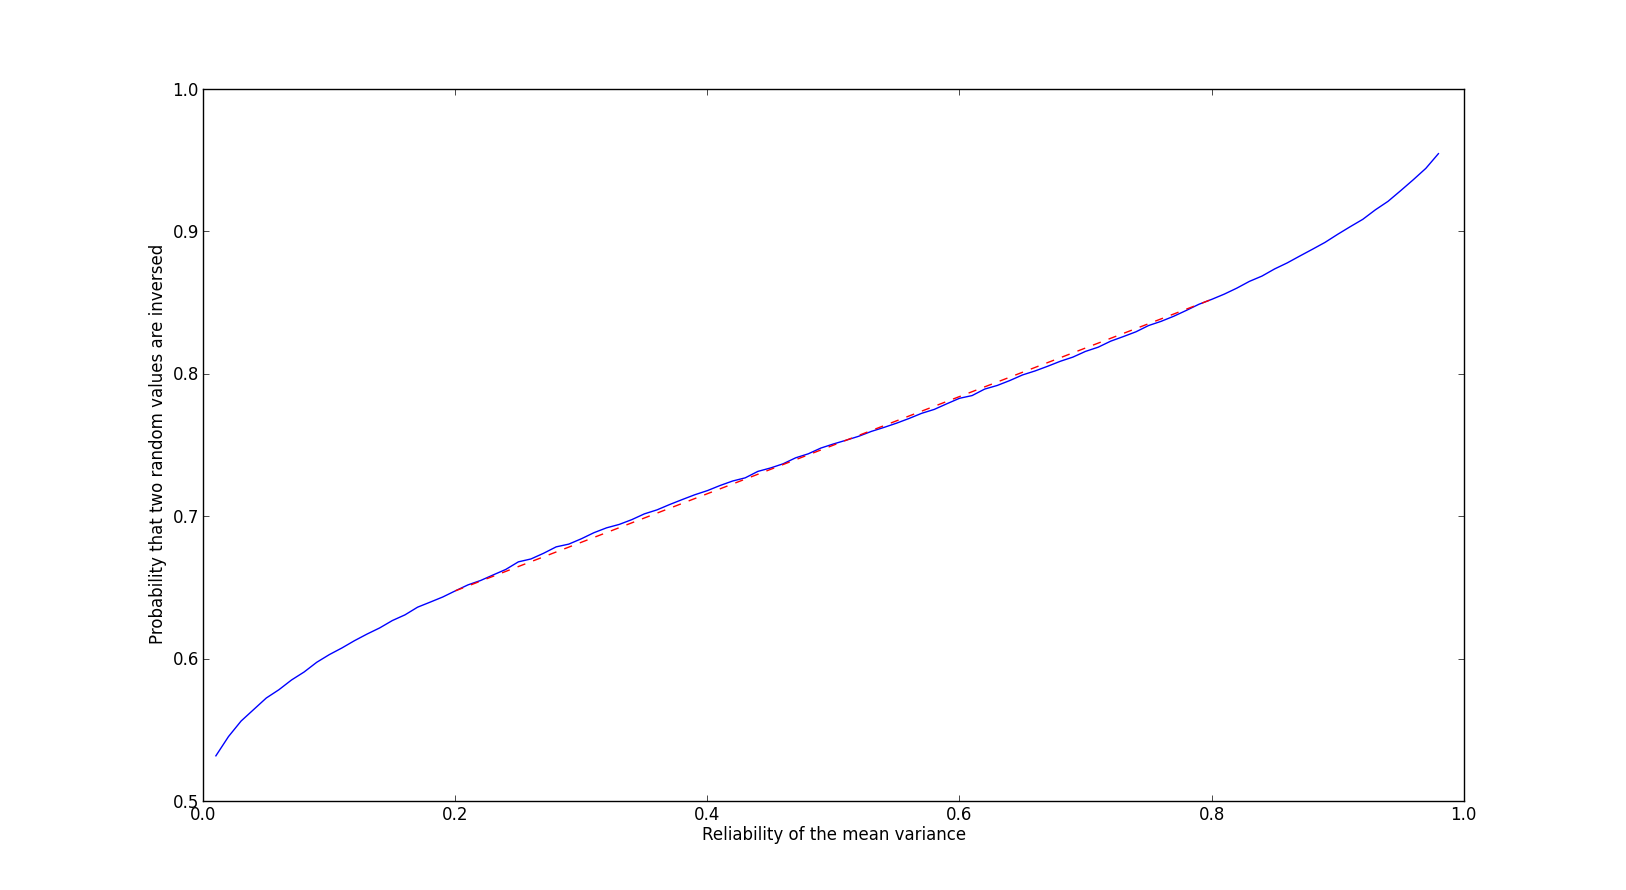
\includegraphics[width=\textwidth]{images/reliVSprob2.png}
\caption{Relation between reliability and percentage of correctly distinguished parameters}
\label{fig:reli}
\end{figure}

When considering the consistency of parameters, a good way to look at them is distinguishability. For example, if we were to look at every possible pair of parameters, in how many cases would the one that is seemingly largest, actually be the largest? The reliability over the average variance of a parameter type is directly related to this measure (see figure \ref{fig:reli})
\end{comment}

\subsection{Data cleaning}
\label{sec:cleaning}
Splitting the data may exacerbate some of the issues that can be encountered in fitting the model. One example is when all questions associated with a student or a KC are answered correctly or incorrectly. This makes the fitting algorithm want to assign infinite values to parameters. Another problem is when for a KC there is such a limited number of questions answered that learning rates cannot be estimated.

To prevent these issues the following steps are taken. On the whole dataset, students that answer all questions correctly or incorrectly are removed. This is after having put the last 7 observations in the testset, which means that students who answered less than 9 questions were all dropped from the data. 
In every split, KC's for which every question is answered correctly or incorrectly is not taken into account for that split. Additionally if for a KC there is less than two questions answered correctly or incorrectly that KC is not taken into account for that split. This means that this KC is removed from the items and any item that no longer contains a KC is dropped from the data. This is done iteratively until the data adheres to these conditions.


\subsection{Domains}
\label{sec:domain}
In generating the data there are many other factors that might play a role in the performance of the models. Among those factors are the values that the parameters will be given, the distribution of knowledge components over the items, the ratio of students to items etc. As indicated in section \ref{sec:RQ} these factors are not explored methodically and extensively, but rather a few different datasets are used to represent some of the variation naturally found in this kind of data. The different datasets and some of the characteristics are described in this section.

\subsubsection{Bridge to Algebra}
The first data-set is one of the datasets used in the 2010 KDD cup on education data mining. The data is from Carnegie Learnings' Cognitive Tutor Software meant for high school-students aged 15-18. \cite{ct} provides an overview of some of the features of this program. The data was obtained from the Bridge to Algebra course during the school year 2006-2007 \cite{bridge}. This dataset will be referred to as the Bridge dataset.

\subsubsection{Algebra I}
This dataset was also provided in the 2010 KDD cup. The data is also obtained from Carnegie Learnings' Cognitive Tutor Software, but from the Algebra I course during the school year 2005-2006 \cite{algebra}. This dataset will be referred to as the Algebra dataset.

\subsubsection{Assistment}
This dataset is quite different from the other two as it is taken from a web-based ITS named Assistment whose details and development story can be found in \cite{razzaq}. The data is from 12 to 14 year old students and was used in \cite{ktpfa} which was discussed in section \ref{sec:RW}. The data does not only contain data from usage of the ITS but also data from a pre-test. This dataset will be referred to as the Assistment dataset.

\subsubsection{Data information}
\begin{table}
    \begin{tabular}{| l | l | l | l |l|}
    \hline
    Dataset & \# questions & \# KCs(cleaned) &\# students(cleaned) & \% correct (testset) \\ \hline
    Bridge & 1,814,398 & 455(34) & 1129(17) & 83 (80)\\ \hline
    Algebra & 585,557 & 104(6) & 564(10) &  76 (75)\\ \hline
    Assistment & 110,842  & 106(0) & 425(20) & 65 (59)\\
    \hline
    \end{tabular}
\end{table} 
   
\begin{table}
	\begin{tabular}{| l | l | l | l |l | l |}
    \hline
    Dataset & 1 & 2 & 3 & 4 & 5-7\\ \hline
    Bridge & 1801254 (0.993) & 11406 (0.006) & 1623(0.001)&113(0.000)&2(0.000) \\ \hline
    Algebra & 368875(0.630)  & 114600 (0.196) & 85818 (0.147)&5581 (0.010)&10683 (0.018) \\ \hline
    Assistment & 56521 (0.510) & 37356 (0.337) & 11770 (0.106) & 4237 (0.038)&958 (0.009)\\
    \hline
    \end{tabular}
\end{table}  

\begin{comment}
2(0.000)& 0&0
6455 (0.011)& 4123(0.007)&105(0.000)
958 (0.009)&0&0
\end{comment}

\begin{comment}
\subsection{KC Experiment}
\subsubsection{The Experiment}
In detail the experiment for KC parameters consists of the following steps per model:
\begin{enumerate}
\item Clean the data by removing students according to section \ref{sec:cleaning}
\item Split the data in a increasing number of parts. Then for each part:
\begin{enumerate}
\item Clean the data by removing KCs according to section \ref{sec:cleaning}
\item Train the model and determine the variance for every parameter type
\item Determine performance on the test-set for that split
\item Determine the inherent variance through the Fisher matrix and through simulation
\item Normalize the found variances with the variances per parameter type found above
\end{enumerate}
\item Determine the variance per parameter over all the splits
\item Normalize the found variances with the average of variances per parameter type found above
\end{enumerate}
\end{commment}
\subsubsection{Representing the Results}
\begin{comment}
Dit is een voorstel voor het representeren van de resultaten. Feedback, ideeen of suggesties worden erg gewaardeerd.
For every split into a number of parts and every model the following will be represented:
\begin{enumerate}
\item The average reliability for each parametertype (both inherent and observed \todo{ preferably the reliability of the difference between the two as well, even though that has not worked too well in the testrun I have shown, although I'm less than 90\% sure I did not make a mistake})
\item The average accuracy and normalized log likelihood
\item Histograms that display the reliabilities of the different parameters. Outliers can now be easily spotted.
\end{enumerate}
\todo{I'd also like to see to what extent inherent and total variance are related over the different splittings and models, as well as relations with accuracy and normalized log likelihood. correlation or spearmans R are two options I'm considering}
\end{comment}

\section{results}
\subsection{Orderings within parameters}
In figure \ref{fig:ranks} the results on first glance are generally as is expected: the tau of parameters improves as more data is used and the rank orders of simulated data are higher than those over splits of observed data. At a second look a few things stand out. Sometimes there seems to be some noise in the experiments (for example the $\eta$ parameter in the Algebra dataset). Furthermore the increase in tau for $\rho$ is small, if existent at all, for the tau over simulated data. Another interesting observation is that the rank orders on the observed data get closer to the rank orders of the simulated data as more data is used and that the gap between the two is smaller for $\beta$ than it is for the learning parameters. Finally it would seem that there is still room for improvement for Tau when adding more data.

\begin{figure}

\centering
\subfloat[Legend for the figures]{
  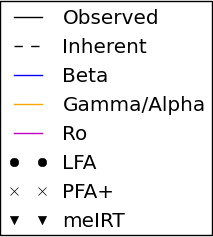
\includegraphics[width=30mm]{images/legend.png}
}
\subfloat[Rankorders for Bridge0506 parameters]{
  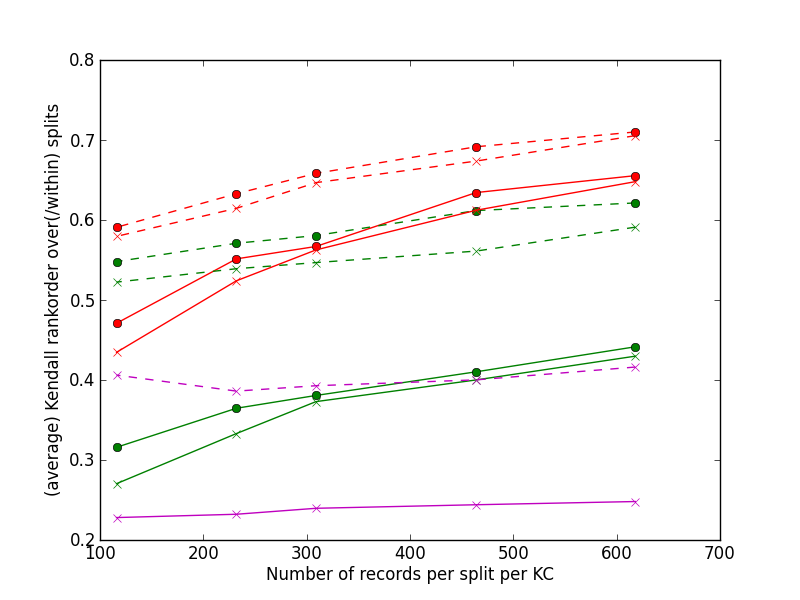
\includegraphics[width=65mm]{images/bridgeallmodranksKC.png}
}
\hspace{0mm}
\subfloat[Rankorders for Algebra0607 parameters]{
  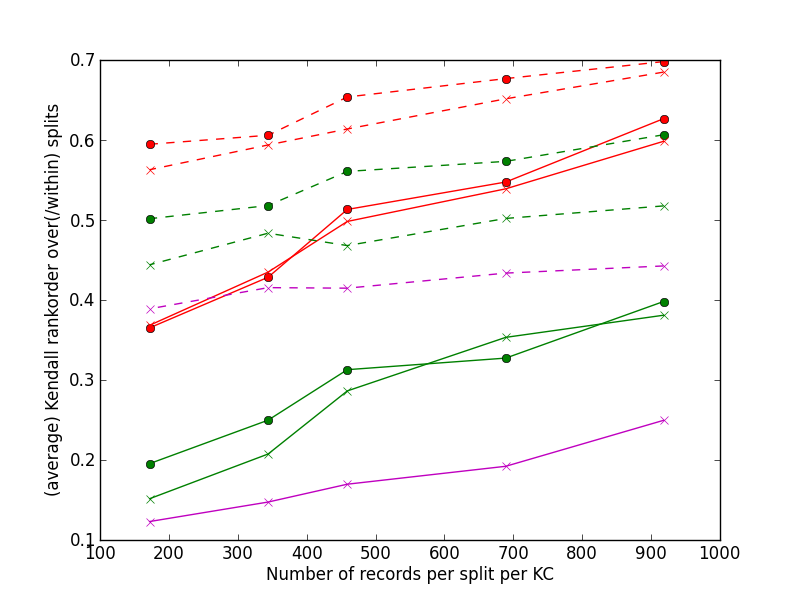
\includegraphics[width=65mm]{images/algebraallmodranksKC.png}
}
\subfloat[Rankorders for Assistment parameters]{
  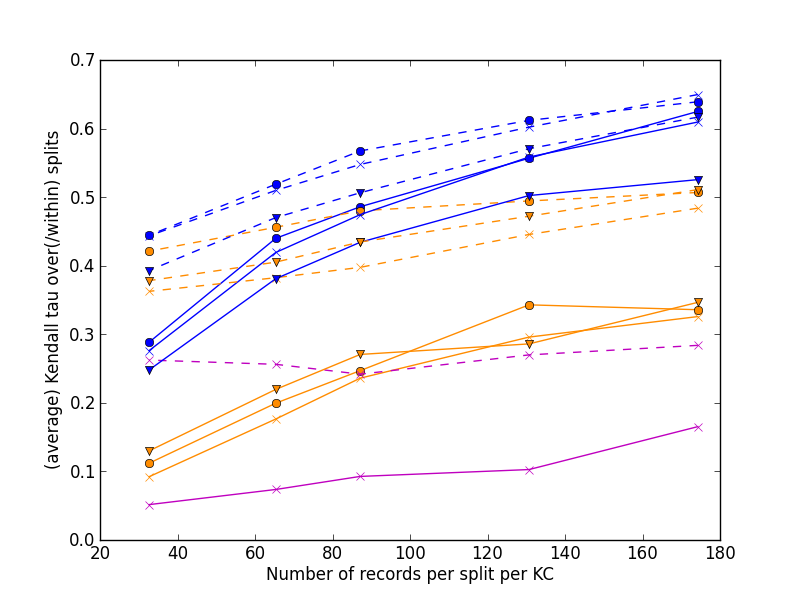
\includegraphics[width=65mm]{images/gongallmodranksKC.png}
}
\caption{Kendall's Tau rank orders of the different parameter-types}
\label{fig:ranks}
\end{figure}

In comparing the LFA and PFA models the rank orders of the $\beta$ parameters, and those of the $\eta$ and $\gamma$ parameters of both models are near each other. It is against expectations that the $\gamma$ parameters rank orders are so high as a simple expectation would be that both $\gamma$ and $\rho$ parameters would show lower rank orders as there is fewer data available per parameter value.
 
The $\tau$ for the different domains look quite similar, which is surprising given the differences in the amount of data per KC for the different domains. The improvements in Tau for the Bridge data set seem to taper off towards the end and will probably benefit least from more data, while the other models still seem to have improving tau values. 
\subsection{Overall variance of parameters}
\label{sec:varresults}
\begin{figure}[!htbp]
\centering
\subfloat[Legend for the figures]{
  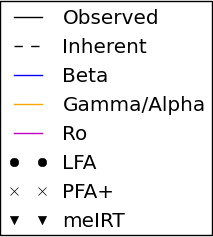
\includegraphics[width=30mm]{images/legend.png}
}
\subfloat[Standard deviations for Bridge0506 parameters]{
  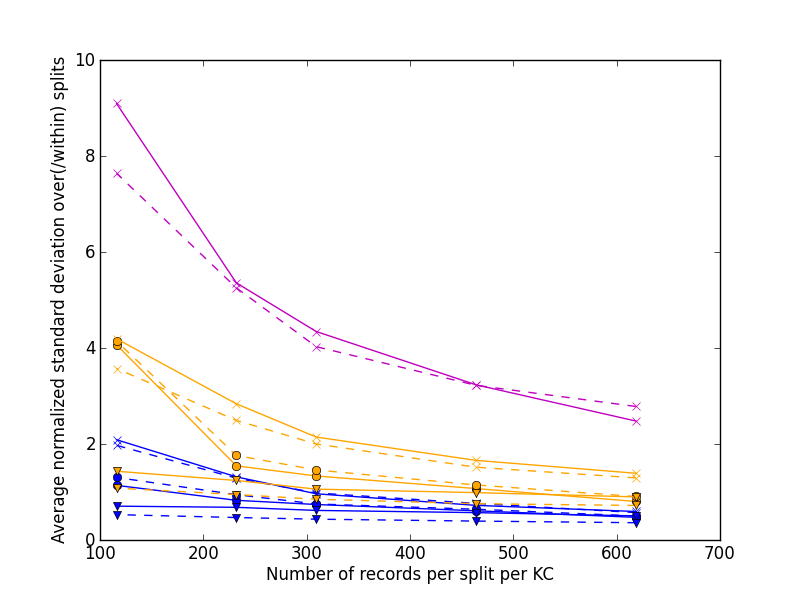
\includegraphics[width=65mm]{images/bridgeallmodsdsKC.png}
}
\hspace{0mm}
\subfloat[Standard deviations for Algebra0607 parameters]{
  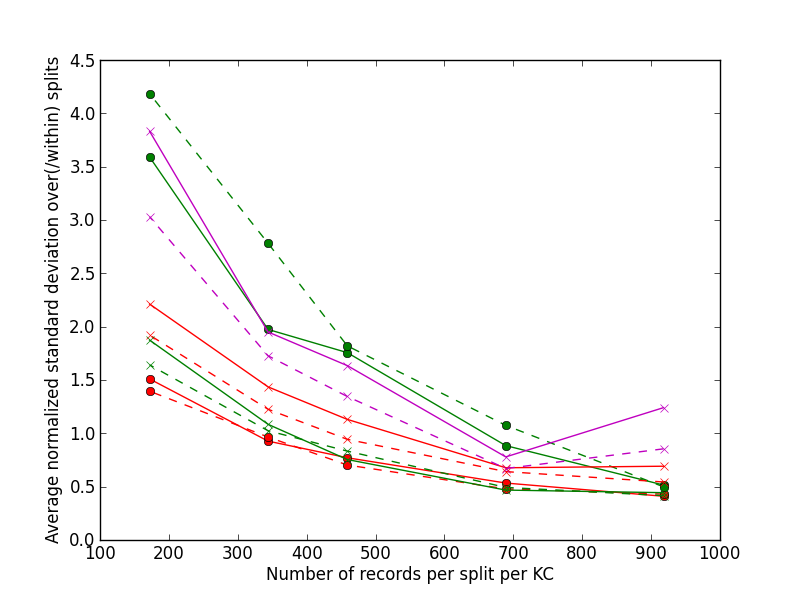
\includegraphics[width=65mm]{images/algebraallmodsdsKC.png}
  \label{fig:sdalg}
}
\subfloat[Standard deviations for Assistment parameters]{
  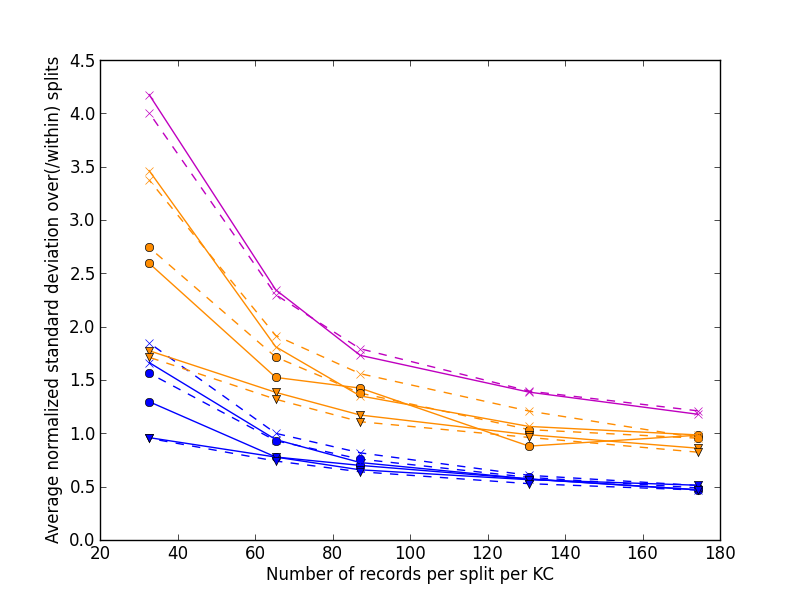
\includegraphics[width=65mm]{images/gongallmodsdsKC.png}
}
\caption{(Average) standard deviations of the different parameters}
\label{fig:sds}
\end{figure}

Figure \ref{fig:sds} is similar to figure \ref{fig:ranks} except with standard deviations over the different splits or generated data sets instead of Kendall's Tau. The diminishing standard deviations are as expected, but both the large values as well as the small difference between variance over splits and variance over generated data sets is surprising given the graphs in figure \ref{fig:ranks}. 

The first might be explained if the different splits give very different parameter values while still largely remaining the same ordering. The second problem would still not be explained though. Upon inspection it turns out that somehow the variation within a parameter of a model fitted on a split is far larger than that of a model fitted on the whole dataset (which was used to normalize the standard deviation values). Additionally the variance within a parameter of a model fitted on generated data is again larger than that of a model fitted on the split used in generating the data. This makes that the same variance has less influence on the ordering since the nearest values of other parameters are further away. Here also lies the explanation for the out-lier of $\rho$ in figure \ref{fig:sdalg}: upon inspection, a model fitted on one of the six splits and its simulated data showed an unusually high standard deviation for $\rho$, having a big impact on the final standard deviations (as was mentioned in section \ref{sec:splits}).

\todo{Ik heb deze data in een onhandig formaat en zou het kunnen agregeren en weergeven om een beter beeld te hebben van hoe dit er precies uitziet en varieert per dataset/parameter/aantal splits}

\subsection{Measures of fit}
In figure \ref{fig:likely} the points belonging to the different splits can easily be distinguished: there are three groups one for each data set (from left to right, Assistment, Algebra and Bridge) and within each group the point with the highest tau value is the one with the most data associated with it. That the PFA models have a higher likelihood is to be expected as it has more parameters than the LFA models. It is also sensible that with more data in a split the likelihood goes down, since the same number of parameter values is used to explain more data. Although there is a nice relationship between tau and likelihood within each dataset, this relationship probably stems from the previous two relationships mentioned: as the amount of data goes up, so do the tau values and as the amount of data goes up, the likelihood goes down. When looking over all three datasets there actually seems to be a slightly positive relation between likelihood and tau values. The wide spread of $\tau$ values over splits of the same dataset (where the relation is quite negative) compared to the slight positive relation makes it unlikely that likelihood can be used to make inferences about the distinguishability of parameter values.   

\begin{figure}[!htbp]
\centering
\subfloat[Average Log Likelihood vs Kendall Tau over splits]{
  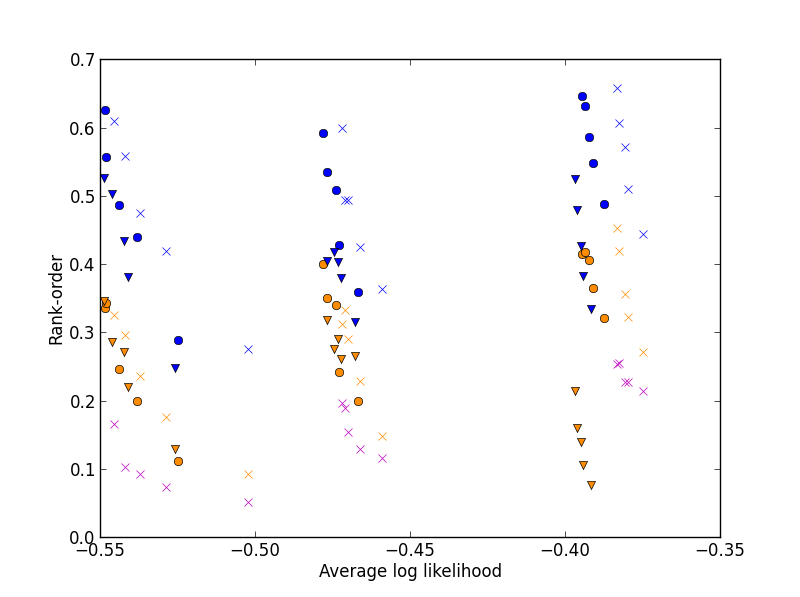
\includegraphics[width=65mm]{images/alllikely.png}
  \label{fig:likely}
}
\subfloat[a' vs total Kendall Tau over splits]{
  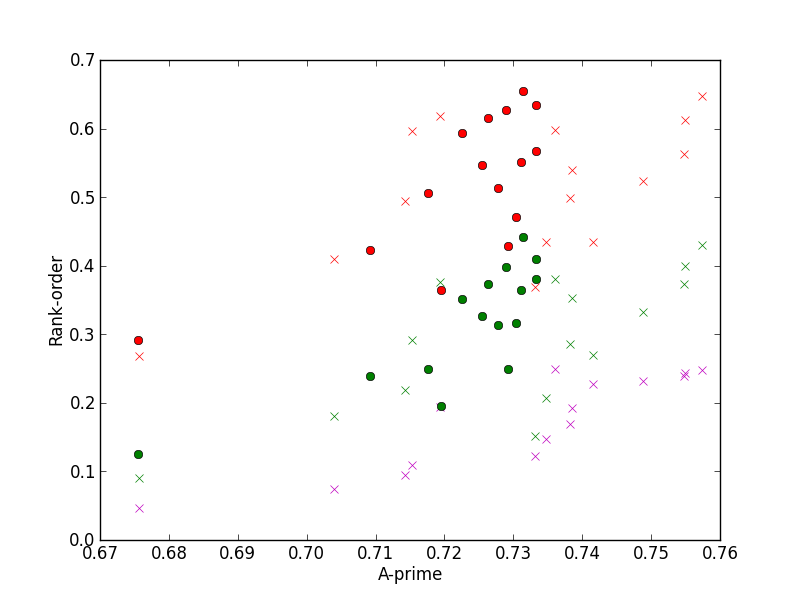
\includegraphics[width=65mm]{images/allaprimes.png}
  \label{fig:ap}
}
\caption{Kendall Tau values vs goodness of fit measures}
\end{figure}

A' shows more promise to be a useful feature in establishing the invariability of parameter values. As seen in figure \ref{fig:ap} there is a positive relation between A' and the tau of all the different parameters in both models. Another interesting observation is that the PFA models generally performs better on A' than the LFA models do.

\subsection{Micro level}
So far the results have been looked at on a global level, now it is time to look at the data from the perspective of individual parameter values. In table \ref{tab:intorank} the Spearman's r values can be seen when comparing the inherent variances and the observed variances of all the different parameter values from all the different splits. The values found are quite high, indicating that inherent variance could well be used in predicting the variance of specific parameter values. 

In section \ref{sec:varresults} it was discovered that over the different splits there can be a significant difference in the variance of a parameter. This has as an unintended consequence that the Spearman's r values are higher when the values of the different splits overlap less. Therefor the Spearman's R values were recalculated using the average of the values in each split rather than the value over all splits combined. The results were vary similar (mostly a difference of .01) and therefor left out. 
\begin{center}
\begin{table}[!htbp]
\begin{tabular}{| l || l | l ||l|l |l|}

    \hline
     & LFA  & & PFA & &   \\ \hline
    Dataset & $\beta$ & $\eta$ & $\beta$ & $\gamma$ & $\rho$  \\ \hline
    Bridge     & .86 & .92 & .91 & .95 & .92 \\ \hline
    Algebra    & .91 & .97 & .94 & .98 & .96 \\ \hline
    Assistment & .90 & .97 & .88 & .97 & .96 \\ \hline \hline
    Overall    & .87 & .94 & .91 & .96 & .94 \\
    \hline
\end{tabular}
\caption{Spearman's R of inherent and total variance of various parameters and models over all splits}
\label{tab:intorank}
\end{table}
\end{center}

\todo{
I have made graphs scatterplotting value in the mainmodel against both inherent variance found in the splits and the observed variance over the splits, but am not sure to include them as I'm not quite sure what I would have liked to learn from them. Interesting observation though is that variance doesn't appear to be higher on the edges.
Interesting still might be to see how such a figure compares to seeing the inherent variance based on the model on whole the data instead of the splits.}

\newpage
\section{Conclusion and Discussion}

In relation to the first subquestion on the influence of the amount of data on the distinguishability of the parameters, the main expectation holds: the more data is used, the more stable the found parameter values and thus distinguishable the parameters become. The improvements made improve less and less as the amount of data is increased. Most parameters ranks, both obtained from the splits and obtained from simulated data are still increasing at the least number of splits used. The exception to this seems to be the $\rho$ parameters in the Bridge dataset where especially for the parameter in the generated case there is barely any improvement. It should be noted that the sizes of the biggest splits already contain a lot of data and that increasing the data further might hide that some parameters can strongly vary in different situations. For example a learning parameter value for a KC that is double the value for one class of students compared to another might show great instability when taking small splits. When splits become very large and students are about equally represented in each group the instability of the learning parameter values disappears as in all splits the same average is found. In IRT it is this kind of variability that is looked out for and can be used to actually improve models when outliers are found.

When looking into the second subquestions of the differences between the domains, the biggest difference is that similar results are obtained on different amounts of data. A possible explanation for this might be that a different definition of size should have been used (e.g. records per parameter value in the model, or counting questions where two KCs are involved as two, where three are involved as three, etc.). Another interesting observation is that in the Assistment dataset the tau on observed data and generated data are relatively near eachother, suggesting that the Assistment domain works more like the model than the other two do.

For the third subquestion it was looked at whether the A' of the test-set or the average likelihood of the data might be indicative of the distinguishability of the parameters. Likelihood of the model in the end is quite unrelated to the tau of the parameters. There seems to be enough of a relation between A' and distinguishability for A' to be of use. Nevertheless the variety in tau values seen around the same A' values show that using A' alone would not be accurate.

When looking at the A' and likelihood values, this is considering how well the model fits on a macro level. To see if something more could be said about individual parameters as well, the rho rankorder values between the variances over the splits and the variances found on generated data was looked at. Since the rho values are quite high it indicates that the variance over the generated data is a good candidate for predicting the real variance over the parameter. A high rho value doesn't guarantee that a good function can be found to relate the two. More research would thus have to be done to establish this. When fitting a function attention could also be paid to investigating if outliers might be caused by bad KC's or items which could be used to improve the Q-matrix or otherwise make discoveries.

For the fourth question the inherent variance was inspected to see what part of the indistinghuisability of the parameter values would result from the stochastic nature of the model. It turns out the stochasticity of the model can often explain a large part of the variation in parameter value orderings. Especially for $\rho$ it shows a rather poor result. 

Finally the observation that variance is of parameters is higher in smaller datasets is disconcerting. It would be a good idea to look at speed of learning over the different splits to see if they are consistent. Otherwise the model would seem to be unfit for estimating levels of students.

In conclusion there is good indication that the distinguishability of parameters, both on a macro level and a micro level might be identified. Nevertheless only the $\beta$ parameters seem to be fairly distinguishable while the learning parameters are marginally distinguishable. Especially the $\rho$ parameter does badly in this regard en when looking at small improvements made by increasing the amount of data, this will not be remedied by using more data. Seeing that the PFA+ models consistently obtain better A' metrics than their LFA counterparts, Gong et al.'s observation that PFA is better for predicting students answers (see section \ref{sec}) seems to extend to PFA+. For student modelling with consistent parameters LFA is more suited than PFA+, even though learning still poses a problem for this model as well and student intitial knowledge needs to be further investigated.



\newpage
\todo{
\section{Things to add and change}
\begin{itemize}
\item Describe terms and use those consistently!
\item related work is a bit out of place as it is not very intelligible without information given later. Maybe move it to the end, or rather integrate it with other stuff?
\item Investigate some of the outliers? 
\end{itemize}
}
\bibliographystyle{alpha}   % this means that the order of references
			    % is determined by the order in which the
			    % \cite and \nocite commands appear
\bibliography{litlist}
\newpage
\appendix
\section{Implementation and Mathematical argumentation}
\label{app:math}
The LFA and PFA models are relatively straightforward in their data representation and implementation. For these models $x$ in formula \ref{eq:logistic} is linear in the parameters, which means that standard logistic regression can be applied. In this appendix first the way the data is represented is described followed by a proof that logistic regression indeed finds the parameter values where the likelihood of the data is highest. 
\subsection{Data Representation}
For logistic regression the data is represented in a matrix $\Phi$ such that $\Phi w$ is equal to a vector of each value of $x$ in formula \ref{eq:logistic}, where $w$ is a column vector of the parameter values. 
In this matrix the rows represent data points while the columns represent what the parameters should be multiplied with. The dimensions of the matrix are thus equal to the number of data points by the number of parameters.

In the formulas for the LFA model (formula \ref{eq:afm}) and the PFA model (formula \ref{eq:pfa}) $x$ consists of a sum where every part contains exactly one parameter. This makes construction of $\Phi$ straightforward: in each row (thus for every data point) a 1 is placed for every present parameter that stands isolated (this goes for $\theta$ and $\beta$) and for the others ($\eta$,$\gamma$ and $\rho$) the right value for that data point is inserted (a non-negative integer). Any parameter not used for that specific datapoint will have a value of 0.

\subsection{Workings of Logistic Regression}
Logistic regression estimates the values of the parameters that maximize the likelihood of the data given the model. The likelihood of the data is equal to $\prod_{d \in D} P_{d}^{t_d}  (1- P_{d})^{1-t_d} $. Here $D$ is the set of all data points and $t_{d}$ is the label (0 for incorrect, 1 for correct) of data-point $d$. The logarithm of this function is taken as this will retain a maximum at the same parameter values, while being easier to derivate since we now have a sum instead of a product. Finally the negative of this log likelihood is taken as this is slightly easier to work with, which results in a minimum being looked for rather than a maximum. The function is then $-\sum_{d \in D}(t_{d} ln(P_{d})+(1-t_{d}) ln(1-P_{d})$.

The first step in finding a solution to this minimization problem is taking the first derivatives of this function in all the parameters. The logistic function has the practical characteristic that its derivative in $x$ is $\sigma (x) (1- \sigma(x))$. The whole derivision can be seen in formula \ref{eq:der1}. Here $\phi_{d}$ is the data for data-point $d$ and is introduced as the derivatives of $x$ in all the parameters. This is possible as $x$ is a linear function in all the parameters. The second to last step is only possible since t can only be 1 or 0. 


\begin{equation}
\label{eq:der1}
\begin{split}
-\sum_{d \in D}(t_{d} \frac{1}{P_{d}} P_{d} (1-P_{d})\phi + (1-t_{d}) \frac{1}{1-P_{d}}(1-P_{d}) (1-(1-P_{d}))(-1)\phi_{d}) &=  \\
-\sum_{d \in D}(t_{d} (1-P_{d})\phi + (1-t_{d})(1-(1-P_{d}))(-1)\phi_{d}) &= \\
-\sum_{d \in D}(t_{d} (1-P_{d})\phi + (1-t_{d})(-P_{d}))\phi_{d}) & = \\
-\sum_{d \in D}(t_{d}-P_{d})\phi_{d} &= \\
\sum_{d \in D}(P_{d}-t_{d})\phi_{d} &
\end{split}
\end{equation}



The first derivatives would be sufficient to perform gradient descent, but this introduces the complexity of finding the right step-size (function). The Newton-Raphson method is an alternative, which can find the parameters where all the first derivatives are 0. For Newton Raphson it is necessary to find the derivatives of the functions we are want to reach zero (i.e. we need all the second derivatives, which is the Hessian). The Hessian is straightforward to obtain as \sum_{d \in D}($P_{d} (1-P_{d}) \phi^{T}*\phi$) where $\phi$ is seen as a row vector. Now the second derivative can be written as a single matrix multiplication: $\Phi^{T} R \Phi$ where $R$ is a diagonal matrix with $P_{d} (1-P_{d})$ on the diagonal. Now the Newton-Raphson method can be applied to find a minimum to the -log likelihood of the data.

Simply finding a minimum is not enough. We want to be sure that we actually find the minimum. In the case of logistic regression there is only one minimum and this must thus be the minimum that is found. The reasoning as to why this is true is explained in this paragraph. That the minus log likelihood has only one minimum is because it is a convex function and a convex (twice differentiable) function always has a semi-definite Hessian (and vice versa). For the Hessian to be semi-definite it is required that for any possible real valued vector $x$, $x^{T}Hx\gec 0$. In the previous paragraph it was established that the Hessian in this case is $\Phi^{T} R \Phi$. Taking $a=\Phi x$ we are left with $a^{T}Ra\gec 0$ as the necessary condition for the Hessian being semi-definite. Since the left side of the equation turns into a sum of squares multiplied by elements from R (which are all zero or positive), this equation must hold. The minus log likelihood is thus a convex function and a found minimum must be the global minimum.


\pagebreak 
\section{Glossary}
\todo{
Making a start with using terms consistently, plus I generally feel that a glossary would have helped me greatly in understanding papers etc.}
\begin{description}
\item[Answer]Whether a question was answered correctly or incorrectly
  \item[Item] A problem (step) in the ITS to which a single answer can be given
  \item[Knowledge Component] A skill, piece of knowledge etc. that is associated with one or more items and in which students can have a level of competence (named 'skill' here)
  \item[paramater] A type of parameter used in one of the models (e.g. $\beta$)
  \item[paramater value] The value of a parameter belonging to a specific case (e.g. the value of the $\theta_{0}$ parameter belonging to student number 10)
  \item[Question] An instance of an item, as asked to a single student
  \item[Skill] Level of skill of a single student
\end{description}

\end{document}
